\documentclass{article}

\usepackage{assign}

\setcoursetitle{CS772: Probabilistic Machine Learning}
\setheaddate{October 25, 2017}

\usepackage{array}

\newcolumntype{L}{>{\centering\arraybackslash}m{14cm}}

\begin{document}
\makeheader%

\begin{question}
	
	The conditional distribution of $\vX$ is given below

	\begin{equation}
		X_{nm}	\qsim	\func{\mt{Poisson}}{\vu_n^T \vv_m}	 \quad \quad \forall\, n \in \brac{N}, \forall\, m \in \brac{M}
		\label{eq:xnm}
	\end{equation}

	The priors on the latent variables are given as follows

	\begin{equation}
		u_{nk}	\eq	\func{\mt{Gamma}}{a_u, b_u}
		\label{eq:unkp}
	\end{equation}

	\begin{equation}
		v_{mk}	\eq	\func{\mt{Gamma}}{a_v, b_v}
		\label{eq:vmkp}
	\end{equation} \br%

	\note{I have used the shape-rate representation as opposed to the question} \br%

	Using these, we can write the conditional posteriors for all latent variables. However, we require to define another set of latent variables \br%

	$\forall\, n, m$ and $\forall\, k \in \brac{K}$, define $X_{nmk}$ such that

	\begin{equation}
		X_{nmk}	\sim	\func{\mt{Poisson}}{u_{nk} v_{mk}}
		\label{eq:xnmkp}
	\end{equation}

	\begin{align*}
		\sum_{k = 1}^K X_{nmk} = X_{nm}
	\end{align*}

	\begin{qsection}{Local Conditional Distributions}

		\begin{qsubsection}{Distribution for $X_{nmk}$}

			We have already been provided with the conditional distrubution of this latent variable as a multinomial distribution

			\begin{equation}
				\set{X_{nmk}}_{k = 1}^K \pipe X_{nm}	\sim	\func{Multinomial}{X_{nm}, \set{\eta_{nmk}}_{k = 1}^K}
				\label{eq:xnmkpo}
			\end{equation}

		keeping all other latent variables fixed, it is easy to see that the best point estimate of $\eta_{nmk}$ is 
		
		\begin{equation}
			\eta_{nmk} = \frac{u_{nk} v_{mk}}{\vu_n^T \vv_m}
			\label{eq:eta}
		\end{equation}
			
		\end{qsubsection}

		\begin{qsubsection}{Distribution of $u_{nk}$}

			We can write the local conditional of $u_{nk}$ \br%

			\note{I will be removing the terms that are independent of $u_{nk}$ as they can be considered constants when we are considering proportionality}

			\begin{align*}
				\prob{u_{nk} \pipe \set{X_{nmk}}_{m = 1}^M, \set{v_{mk}}_{m = 1}^M}	&\qprop	\prob{\set{X_{nmk}}_{m = 1}^{M} \pipe u_{nk}, \set{v_{mk}}_{m = 1}^M} \prob{u_{nk}} \\
																					&\eq	\prod_{m = 1}^{M} \para{\prob{X_{nmk} \pipe u_{nk}, v_{mk}}} \prob{u_{nk}} \\
																					&\eq	\prod_{m = 1}^{M} \para{\exp{-u_{nk} v_{mk}} \frac{\para{u_{nk} v_{mk}}^{X_{nmk}}}{\fact{X_{nmk}}}} u_{nk}^{a_u - 1} \exp{- b_u u_{nk}} \\
																					&\eq	\exp{-\para{b_u + \sum_{m = 1}^{M} v_{mk}}} u_{nk}^{\para{a_u + \sum_{m = 1}^{M} X_{nmk}} - 1}
			\end{align*}

			This has the same representation as that of a gamma distribution. Hence, upon noramlization, we get
		
			\begin{equation}
				\prob{u_{nk} \pipe \vX, \vv}	\eq	\func{\mt{Gamma}}{a_u + \sum_{m = 1}^{M} X_{nmk}, b_u + \sum_{m = 1}^{M} v_{mk}}
				\label{eq:unkpo}
			\end{equation}
		
		\end{qsubsection}

		\begin{qsubsection}{Distribution of $v_{mk}$}

			This can be solved the exact same way as the distribution for the l.v. $u_{nk}$. Here, we get

			\begin{equation}
				\prob{v_{mk} \pipe \vX, \vu}	\eq	\func{\mt{Gamma}}{a_v + \sum_{n = 1}^{N} X_{nmk}, b_v + \sum_{n = 1}^{N} u_{nk}}
				\label{eq:vnkpo}
			\end{equation}

		\end{qsubsection}
		
	\end{qsection}

	\begin{qsection}{Algorithm for Gibbs Sampling}

		\begin{algo}{h!}{Gibbs Sampling for Count Matrix Factorization}

			Let $T_b$ be the number of samples to be burned and $T$, the number of samples required. Hence we iterate $T + T_b$ times and save the last $T$ samples.

			\begin{itemize}
				\item Initialize $\set{u_{nk}}, \set{v_{mk}}$ (We can also initialize $\set{X_{nmk}}$, however it is redundant, and the samples will be replaced in the first iteration itself)
				\item Do till sufficient samples acquired
					\begin{enumerate}
						\item $\forall\, n \in \brac{N}$, $\forall\, m \in \brac{M}$ and $\forall\, k \in \brac{K}$ sample $\set{X_{nmk}}$ using equation~\ref{eq:xnmkpo}
						\item $\forall\, n \in \brac{N}$ and $\forall\, k \in \brac{K}$ sample $\set{u_{nk}}$ using equation~\ref{eq:unkpo} and using the current samples of $\set{X_{nmk}}$
						\item $\forall\, m \in \brac{M}$ and $\forall\, k \in \brac{K}$ sample $\set{v_{mk}}$ using equation~\ref{eq:vnkpo} and using the current samples of $\set{X_{nmk}}$ and $\set{u_{nk}}$
					\end{enumerate}
			\end{itemize}

		\end{algo}

		\begin{qsubsection}{Sampling from Multinomial}
			To find one sample from a multinomial distribution (say $\func{\mt{Multinomial}}{x; \set{\eta_k}_{k \in {L}}}$), we can do the following

			\begin{enumerate}
				\item Sample $u \sim \func{Unif}{0, 1}$
				\item Find min $\pr{K}$ such that $\sum_{k = 1}^{\pr{K}} \ge u$ and add 1 to $x_{\pr{K}}$
			\end{enumerate}
		\end{qsubsection}
		
	\end{qsection}

\end{question}

\clearpage

\begin{question}

	\begin{qsection}{Plots}
		\begin{figure}[h!]
			\centering
			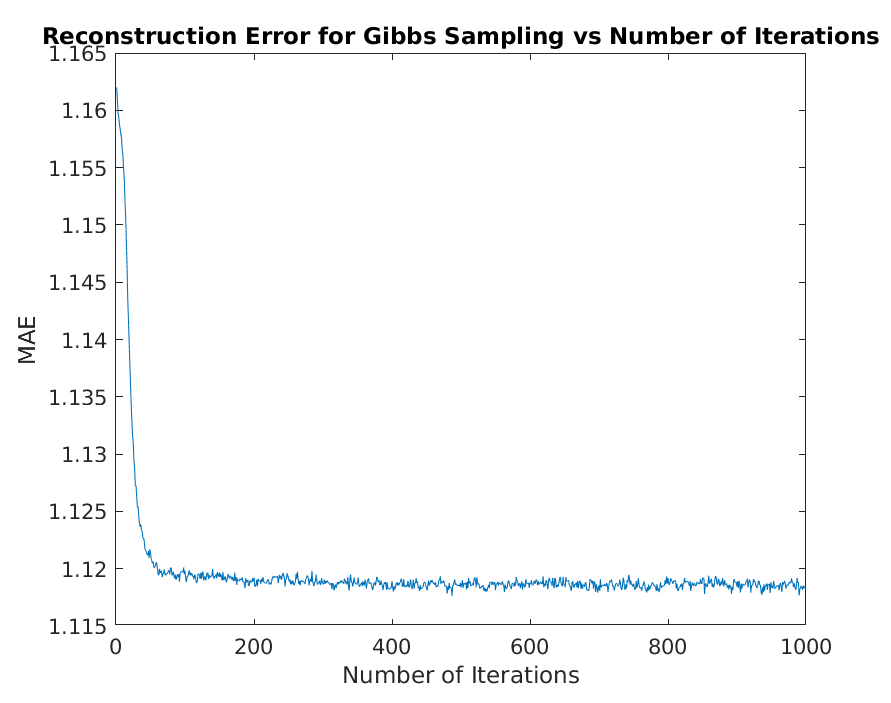
\includegraphics[width=12cm]{plots/gibbs.png}
			\caption{Reconstruction error using Gibbs Sampling}
		\end{figure}

		\begin{figure}[h!]
			\centering
			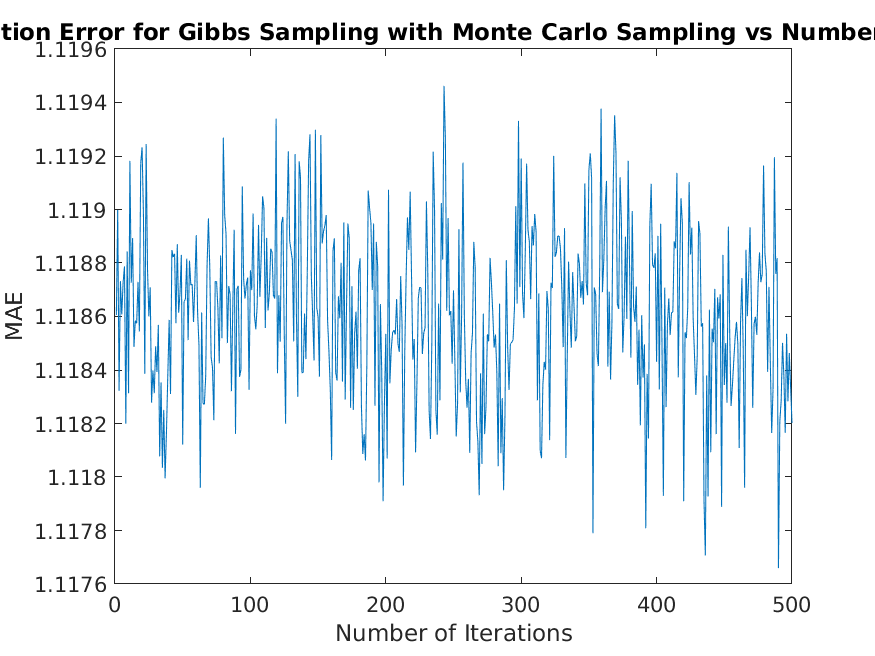
\includegraphics[width=12cm]{plots/gibbs_mc.png}
			\caption{Reconstruction error using Gibbs Sampling along with Monte Carlo estimation}
		\end{figure}

	\end{qsection}

	\begin{qsection}{Observed Clusters of Words}	
		\def\arraystretch{1.8}
		\begin{tabular}[h!]{| c | L |}
			\hline
			\textbf{Cluster ID}	&	\textbf{Words} \\
			\hline
			1	& 	windows window file problem program files run display running screen color set line work graphics version application image sun mit \\
			2	& 	people gun state law government bill writes rights fire guns article make police laws fbi crime don weapons clinton carry \\
			3	& 	car good bike dod cars article don engine buy front acs drive road ride driving ohio riding speed bmw miles \\
			4	& 	key system chip encryption keys government public security clipper information phone secure secret communications nsa data message escrow algorithm bit \\
			5	& 	writes pitt disease ve gordon medical blood read don banks steve pain food treatment medicine study normal patients effect effects \\
			6	& 	interested price sale offer send mail sell shipping call condition ll list email original excellent selling sound includes deal make \\
			7	& 	game year team play games win season hockey players league teams time baseball player san good red division won playing \\
			8	& 	card drive system disk computer video bit mac memory speed software dos hard board problem ram mb drives controller apple \\
			9	& 	writes article apr don cs david ca netcom org steve opinions cc deleted csd mine isc ve good disclaimer stanford \\
			10	& 	net wrote apple ve kent heard cheers sandvik don activities tom private ca great write cs lee dave find article \\
			11	& 	israel article writes israeli people org arab jews opinions don jewish number state peace research virginia palestinian war arabs israelis \\
			12	& 	information number list send mail time program read note data questions info include software code ftp general address free based \\
			13	& 	god people point fact true life jesus christian question things make time read christians word world man good bible person \\
			14	& 	university mail fax internet phone michael email computer bitnet information advance research gatech uk ac georgia tel department technology institute \\
			15	& 	space gov nasa high power earth work low cost sun toronto ground long access pat orbit moon henry small system \\
			16	& 	time back good make didn lot things don thing put people years long bad ve doesn ago point give ll \\
			17	& 	writes keith cwru caltech jon sgi usenet time freenet john cleveland good po find bob don start ago past internet \\
			18	& 	max cs hp part ca fi st de du ed ms ac tm ve bu ut ma al article se \\
			19	& 	writes article uiuc news andrew cso mike cmu uchicago frank hear robert post don curious day michael guy duke isn \\
			20	& 	people years world government country today american states history turkish state children president war military political united press national closed \\
			\hline
		\end{tabular}
	\end{qsection}

	
\end{question}

\clearpage

\begin{question}

	The acceptance rate for different variances are given as below \br%

	\begin{center}

		\def\arraystretch{1.8}
		\begin{tabular}[h!]{p{3cm} p{4cm}}
			\textbf{Variance}	&	\textbf{Acceptance Rate}	\\
			\hline%
			0.01				&	0.973047					\\
			0.01				&	0.359208					\\
			0.01				&	0.007248					\\
		\end{tabular}

	\end{center} \br%

	The means and variances approximated using the samples generated are as follows \br%
	
	\begin{center}

		\def\arraystretch{1.8}
		\begin{tabular}[h!]{p{3cm} p{4cm} p{7cm}}
			\textbf{Variance}	&	\textbf{Estimated Mean}	&	\textbf{Estimated Variance}			\\
			\hline%
			0.01				&	4.1833, 4.0969			&	5.6557, 5.6262; 5.6262, 6.1487		\\
			0.01				&	4.0121, 4.0205			&	0.57950, 0.45151; 0.45151, 0.57677	\\
			0.01				&	4.0019, 4.0069			&	16.595, 16.487; 16.487, 16.632		\\
		\end{tabular}

	\end{center} \br%

	Looking at the data, we can clearly say that $\sigma^2 =$ \textbf{1} is the best value we can obtain, both from the perspective of estimated $\vmu$ and $\vSigma$ as well as the acceptance ratio. We do not need a very low acceptance ratio, as it reduces the diffusion rate a lot, also, very small variance causes a lot of error (Discussed in class).

	\begin{figure}[h!]
		\centering
		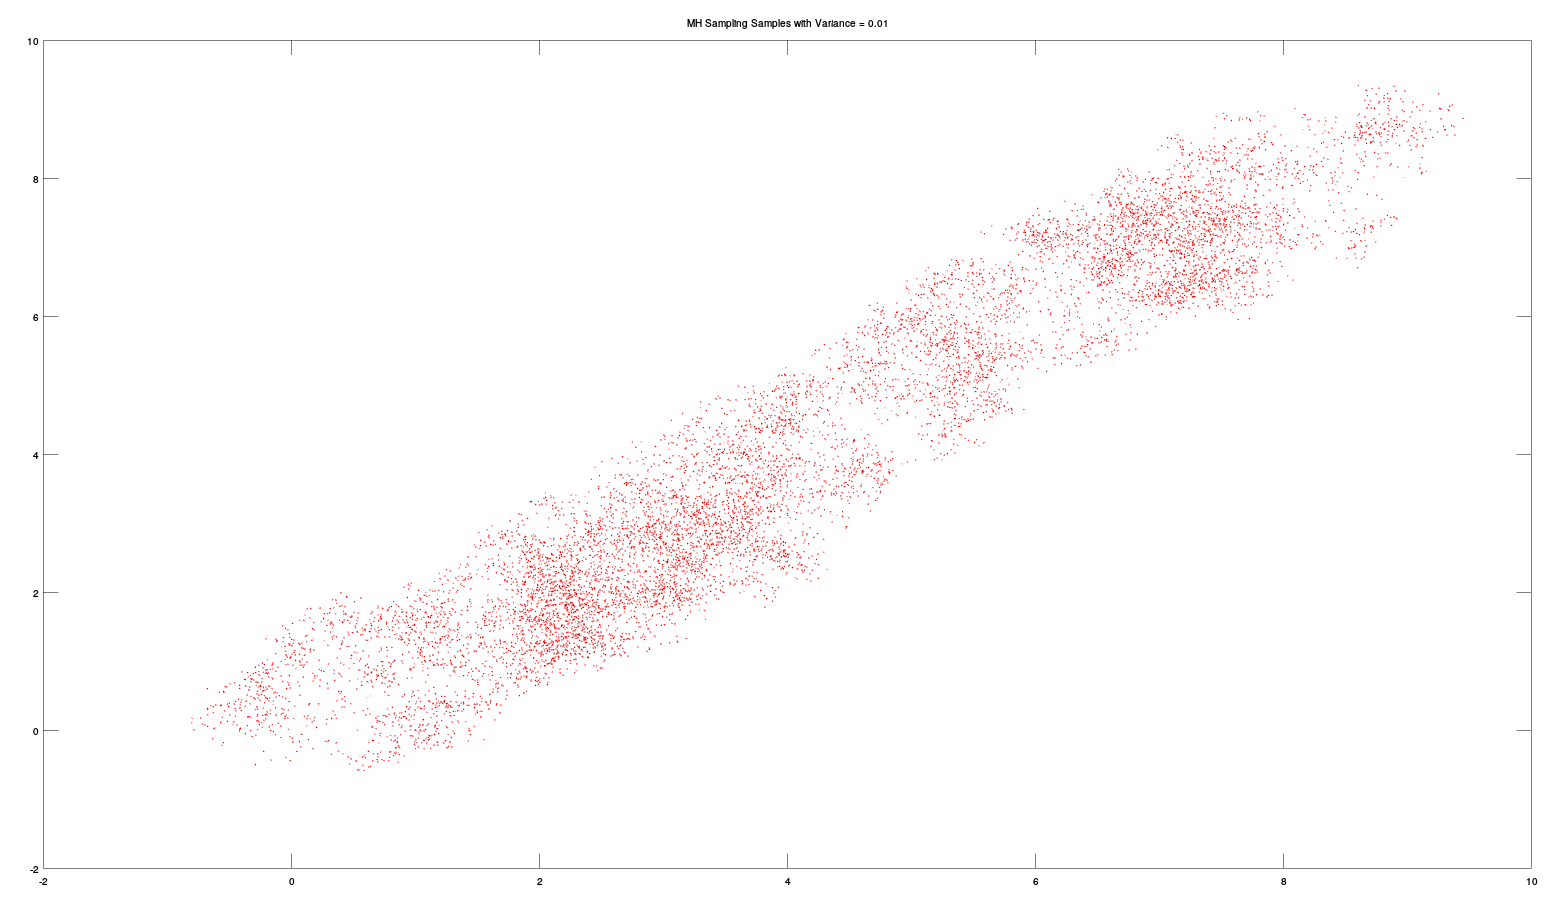
\includegraphics[width=15cm]{plots/samples1.png}
		\caption{Samples obtained using MH Sampling with Variance = 0.01}
	\end{figure}
	
	\begin{figure}[h!]
		\centering
		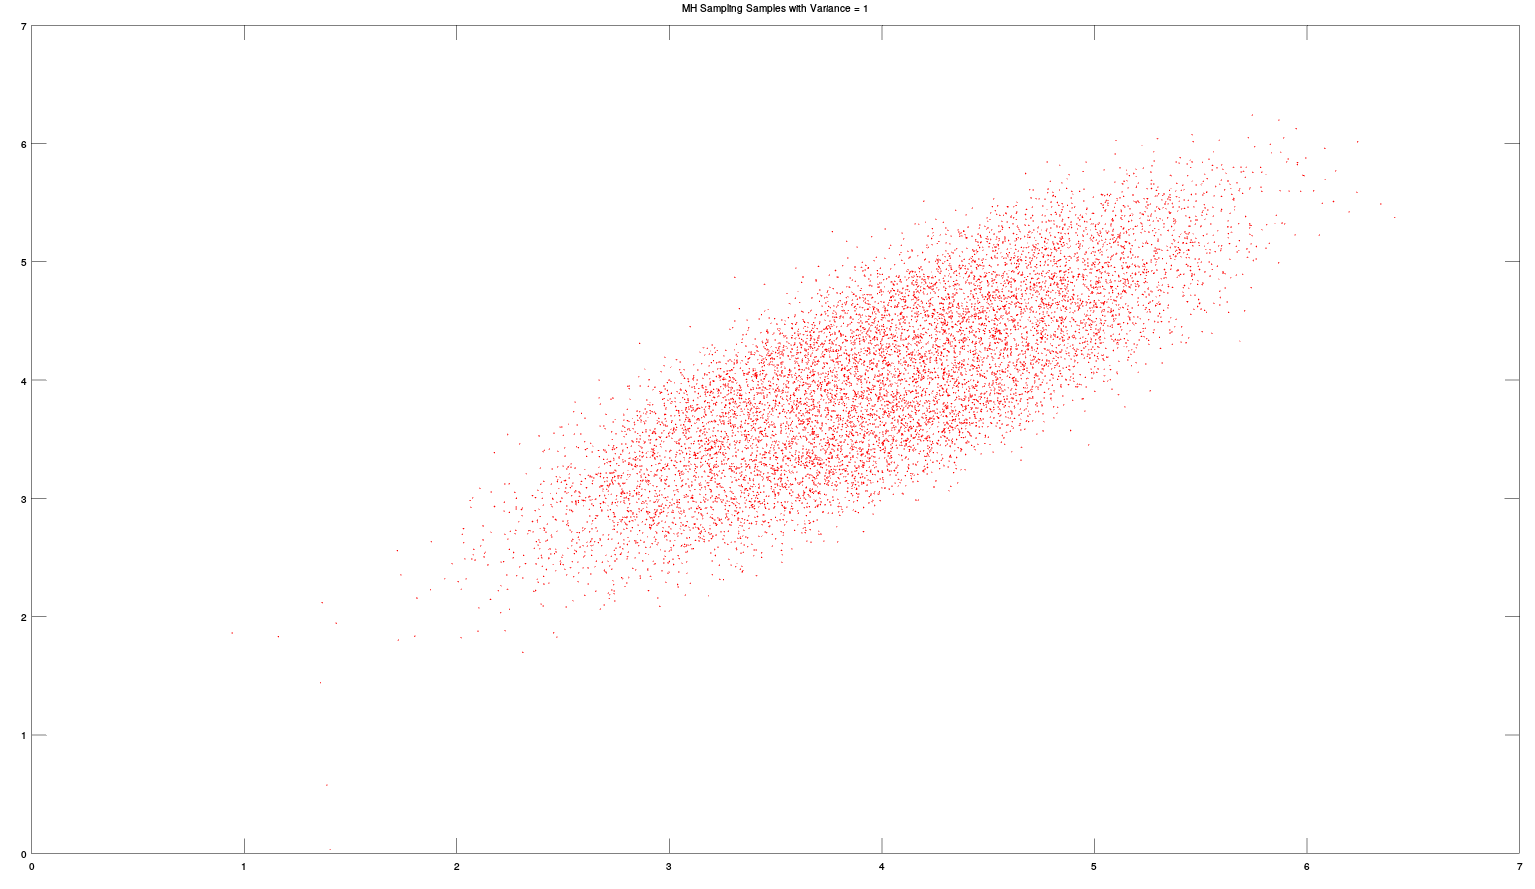
\includegraphics[width=15cm]{plots/samples2.png}
		\caption{Samples obtained using MH Sampling with Variance = 1}
	\end{figure}

	\begin{figure}[h!]
		\centering
		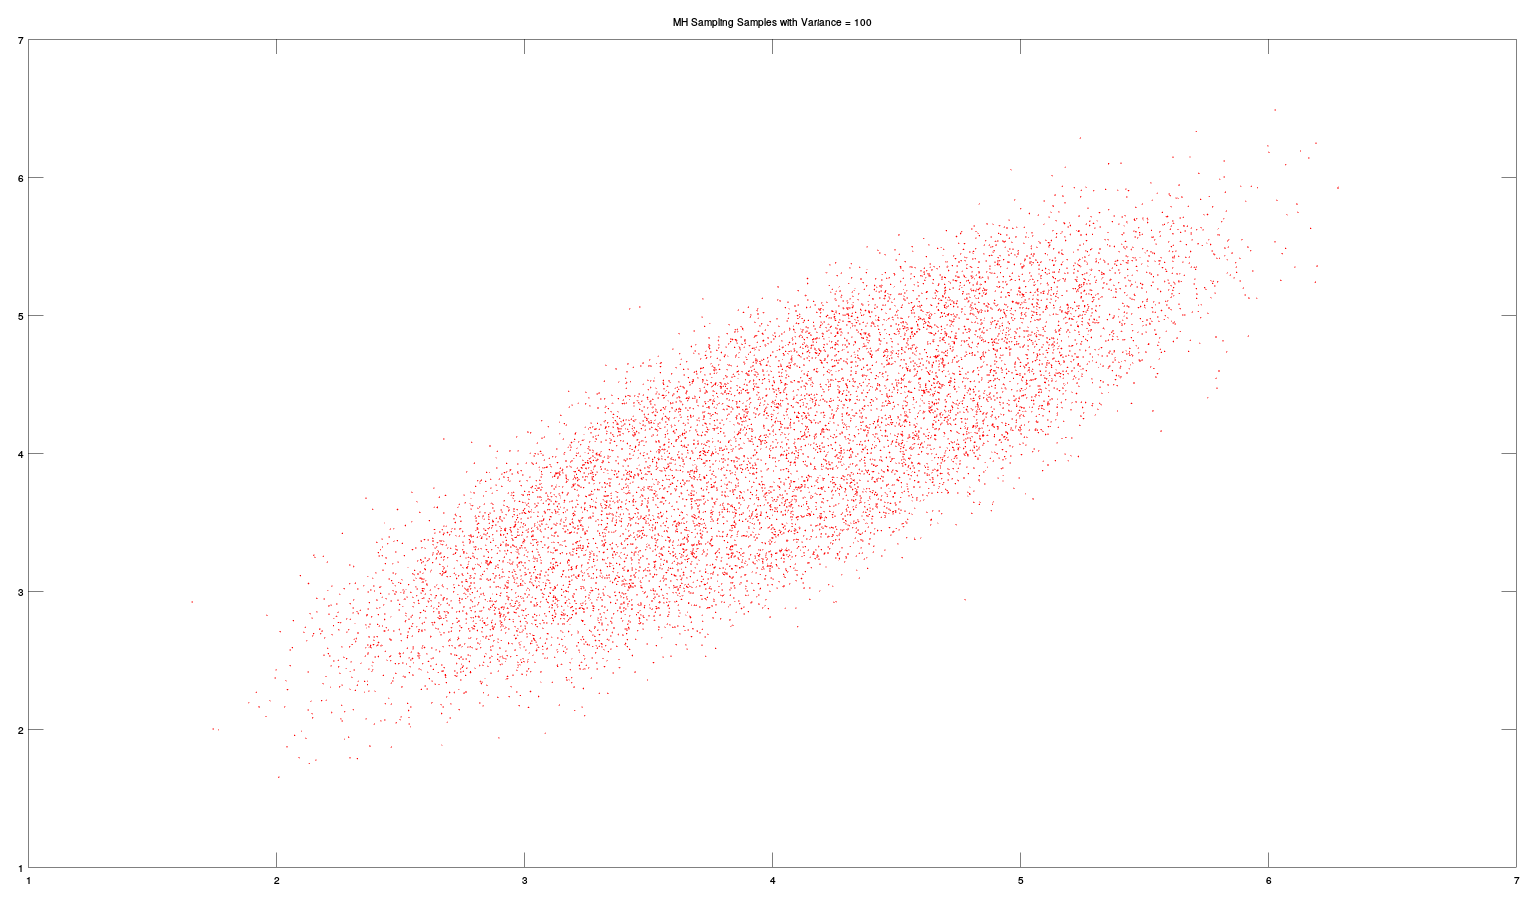
\includegraphics[width=15cm]{plots/samples3.png}
		\caption{Samples obtained using MH Sampling with Variance = 100}
	\end{figure}
\end{question}

\clearpage

\begin{question}
	\begin{qsection}{Notations}

		\begin{tabular}[h!]{p{2cm} l}
			$\vX$			&	Complete set of Data																	\\
			$\vX_{obs}$		&	Set of Observed Data																	\\
			$\vX_{miss}$	&	Set of Missing Data																		\\
			$\vz$			&	Set of Cluster Assignments for all samples												\\
			$\vmu$			&	Set of Cluster Means, with each cluster mean represented as $\vmu_k$					\\
			$\vSigma$		&	Set of Cluster Covariances, with each cluster covariance represented as $\vSigma_k$		\\
			$\vpi$			&	Set of Probabilities of Cluster Assignments 
		\end{tabular}
		
	\end{qsection}

	\begin{qsection}{Complete Log Likelihood}

		Since we require to also model the missing data, we can treat these missing data samples as latent variables. Hence we need to compute the expectations with respect to both $\vX_{miss}$ and $\vz$. \br%

		In order to compute the CLL, we first need to find the joint distribution of $\vX_{obs}, \vX_{miss}, \vz$

		\begin{align*}
			\vx^n \pipe z^n = k, \vmu_k, \vSigma_k	&\qsim	\ND{\vx^n \pipe \vmu_k, \vSigma_k} \\
			\vx^n \pipe z^n, \vmu, \vSigma			&\qsim	\prod_{k = 1}^{K} \para{\ND{\vx^n \pipe \vmu_k, \vSigma_k}}^{\is{z^n = k}} \\
			\vx^n, z^n \pipe \vmu, \vSigma			&\qsim	\prod_{k = 1}^{K} \para{\pi_k \ND{\vx^n \pipe \vmu_k, \vSigma_k}}^{\is{z^n = k}} \\
			\vX, \vz \pipe \vmu, \vSigma			&\qsim	\prod_{n = 1}^{N} \prod_{k = 1}^{K} \para{\pi_k \ND{\vx^n \pipe \vmu_k, \vSigma_k}}^{\is{z^n = k}}
		\end{align*}

		Hence, we can write the CLL (removing terms independent of the latent variables) as

		\begin{align*}
			CLL		&\eq	\log{\prob{\vX, \vz \pipe \vmu, \vSigma}} \\
					&\eq	\sum_{n = 1}^{N} \sum_{k = 1}^{K} \is{z^n = k} \brac{\log{\pi_k} - \frac{1}{2} \para{\vx^n - \vmu_k}^T \vSigma_k^{-1} \para{\vx^n - \vmu_k} - \frac{1}{2} \log{\norm{\vSigma_k}}}
		\end{align*}

		We need to compute the expectation of CLL wrt to the joint posterior of $\vX_{miss}$ and $\vz$. Therefore, we can write the Expected CLL as

		\begin{align*}
			\E{CLL}		&\eq	\sum_{n = 1}^{N} \sum_{k = 1}^{K} \E{\is{z^n = k} \para{\log{\pi_k} - \frac{1}{2} \para{\vx^n - \vmu_k}^T \vSigma_k^{-1} \para{\vx^n - \vmu_k} - \frac{1}{2} \log{\norm{\vSigma_k}}}} \\
						&\eq	\sum_{n = 1}^{N} \sum_{k = 1}^{K} \para{\E{\is{z^n = k}} \log{\pi_k} - \frac{1}{2} \E{\is{z^n = k} \para{\vx^n - \vmu_k}^T \vSigma_k^{-1} \para{\vx^n - \vmu_k}} - \frac{1}{2} \E{\is{z^n = k}} \log{\norm{\vSigma}}}
		\end{align*}

		where the second term can be written as

		\begin{align*}
			\para{\vx^n - \vmu_k}^T \vSigma_k^{-1} \para{\vx^n - \vmu_k}				&\eq	\trace{\vSigma_k^{-1} \para{\vx^n - \vmu_k} \para{\vx^n - \vmu_k}^T} \\
			\implies \E{\is{z^n = k} \para{\vx^n - \vmu_k}^T \vSigma_k^{-1} \para{\vx^n - \vmu_k}}	&\eq	\trace{\vSigma_k^{-1} \E{\is{z^n = k} \para{\vx^n - \vmu_k} \para{\vx^n - \vmu_k}^T}}
		\end{align*}

		We can further distribute the expectation as follows

		\begin{align*}
			\para{\vx^n - \vmu_k} \para{\vx^n - \vmu_k}^T	&\eq	\vx^n {\vx^n}^T - 2 \vx^n \vmu_k^T + \vmu_k \vmu_k^T
		\end{align*}

		Using the trick from the midsem solutions, we can write $\vx^n as \brac{\vx_{obs}^n, \vx_{miss}^n}$, and following the same pattern, we can say that we require the following three expectations
		\begin{enumerate}
			\item $\E{\is{z^n = k}}$
			\item $\E{\is{z^n = k} \vx_{miss}^n}$
			\item $\E{\is{z^n = k} \vx_{miss}^n {\vx_{miss}^n}^T}$
		\end{enumerate}
		
	\end{qsection}

	\begin{qsection}{E Step --- Expectation Calculation}

		\begin{qsubsection}{Expectation --- $\E{\is{z^n = k}}$}

			\begin{align*}
				\E{\is{z^n = k}}	&\eq	\sum_{\pr{k} = 1}^{K} \int \is{\pr{k} = k} \prob{z^n = \pr{k}, \vx_{miss}^n \pipe \vx_{obs}^n, \vmu, \vSigma} d \para{\vx_{miss}^n} \\
									&\eq	\int \prob{z^n = k, \vx_{miss}^n \pipe \vx_{obs}^n, \vmu, \vSigma} d \para{\vx_{miss}^n} \\
									&\eq	\prob{z^n = k \pipe \vx_{obs}^n, \vmu, \vSigma} \\
									&\qprop	\prob{z^n = k} \prob{\vx_{obs}^n \pipe z^n = k, \vmu, \vSigma} \\
									&\eq	\pi_k \prob{\vx_{obs}^n \pipe z^n = k, \vmu, \vSigma}
			\end{align*}

			\note{This is a marginal distribution wrt a multivariate Gaussian and can be easily computed}

			\begin{align*}
				\E{\is{z^n = k}}	&\qprop	\pi_k \ND{\vx_{obs}^n \pipe \vmu_k^n, \vSigma_k^n} \\
			&\eq	\frac{\pi_k \ND{\vx_{obs}^n \pipe \vmu_k^n, \vSigma_k^n}}{\sum_{\pr{k} = 1}^{K} \pi_{\pr{k}} \ND{\vx_{obs}^n \pipe \vmu_{\pr{k}}^n, \vSigma_{\pr{k}}^n}}
			\end{align*}

			\note{$\vmu_k^n$ represents the marginal mean for the observed data sample $\vx^n$, and $\vmu_k^{-n}$ represents the marginal mean for the missing part. Similarly defined for $\vSigma$}
	
		\end{qsubsection}

		\begin{qsubsection}{Expectation --- $\E{\is{z^n = k} \vx_{miss}^n}$}

			\begin{align*}
				\E{\is{z^n = k} \vx_{miss}^n}	&\eq	\sum_{\pr{k} = 1}^{K} \int \is{\pr{k} = k} \vx_{miss}^n \prob{z^n = \pr{k}, \vx_{miss}^n \pipe \vx_{obs}^n, \vmu, \vSigma} d \para{\vx_{miss}^n} \\
												&\eq	\int \vx_{miss}^n \prob{z^n = k, \vx_{miss}^n \pipe \vx_{obs}^n, \vmu, \vSigma} d \para{\vx_{miss}^n} \\
												&\eq	\prob{z^n = k \pipe \vx_{obs}, \vmu, \vSigma} \int \vx_{miss}^n \prob{\vx_{miss}^n \pipe z^n = k, \vx_{obs}^n, \vmu, \vSigma} d \para{\vx_{miss}^n}
			\end{align*}

			This is the expected value of $\vx_{obs}^n$ conditioned on $\vx_{miss}^{n}$. This can be easily computed using the Gaussian properties. We represent this as $\vmu_k^{-n \pipe n}$

			\begin{align*}
				\E{\is{z^n = k} \vx_{miss}^n}	&\eq	\E{\is{z^n = k}} \mu_k^{-n \pipe n}
			\end{align*}
			
		\end{qsubsection}

		\begin{qsubsection}{Expectation --- $\E{\is{z^n = k} \vx_{miss}^n {\vx_{miss}^n}^T}$}

			\begin{align*}
				\E{\is{z^n = k} \vx_{miss}^n {\vx_{miss}^n}^T}	&\eq	\sum_{\pr{k} = 1}^{K} \int \is{\pr{k} = k} \vx_{miss}^n {\vx_{miss}^n}^T \prob{z^n = \pr{k}, \vx_{miss}^n \pipe \vx_{obs}^n, \vmu, \vSigma} d \para{\vx_{miss}^n} \\
																&\eq	\prob{z^n = k \pipe \vx_{obs}^n, \vmu, \vSigma} \int \vx_{miss}^n {\vx_{miss}^n}^T \prob{\vx_{miss}^n \pipe z^n = k, \vx_{obs}^n, \vmu, \vSigma} d \para{\vx_{miss}^n} \\
																&\eq	\E{\is{z^n = k}} \para{\vmu_k^{-n \pipe n} {\vmu_k^{-n \pipe n}}^T + \vSigma_k^{-n \pipe n}}
			\end{align*}
			
		\end{qsubsection}

	\end{qsection}

	\begin{qsection}{M Step --- Maximization Step}

		\begin{qsubsection}{MLE estimate of $\vpi$}

			\begin{align*}
				\hat{\vpi}						&\eq 	\argmax_{\vpi} \E{CLL} \\
												&\quad \quad \quad \quad \mt{s.t.} \sum_{k = 1}^{K} \pi_k \,=\, 1 \\
												&\eq 	\argmax_{\vpi} \E{CLL} + \lambda \para{1 - \sum_{k = 1}^{K}} \\
				\implies \derp{\E{CLL}}{\pi_k} 	&\eq	\lambda	\quad \quad \forall\, k \in \brac{K} \\
				\implies \hat{\pi_k}			&\eq	\frac{\sum_{n = 1}^{N} \E{\is{z^n = k}}}{\lambda}
			\end{align*}

			Using the constraint on $\vpi$, we get

			\begin{align*}
				\hat{\pi_k}	\eq	\frac{\sum_{n = 1}^{N} \E{\is{z^n = k}}}{N}
			\end{align*}

		\end{qsubsection}

		\begin{qsubsection}{MLE estimate of $\vmu$}

			\begin{align*}
				\hat{\vmu}					&\eq		\argmax_{\vmu} \E{CLL} \\
				\derp{\E{CLL}}{\vmu_k}		&\eq		- \frac{1}{2} \sum_{n = 1}^{N} \sum_{k = 1}^{K} \E{\is{z^n = k} \derp{\para{\vx^n - \vmu_k}^T \vSigma_k^{-1} \para{\vx^n - \vmu_k}}{\vmu_k}} 	&\eq	0 \\
											&\implies	- \frac{1}{2} \sum_{n = 1}^{N} \E{\is{z^n = k} 2 \vSigma_k^{-1} \para{\vx^n - \vmu_k}}															&\eq	0 \\
				\implies	\hat{\vmu_k}	&\eq		\frac{\sum_{n = 1}^{N} \E{\is{z^n = k} \vx^n}}{\sum_{n = 1}^{N} \E{\is{z^n = k}}}
			\end{align*}

			where

			\begin{align*}
				\E{\is{z^n = k} \vx^n}	\eq	\begin{bmatrix}
											\E{\is{z^n = k}} \vx_{obs}^n \\\\
											\E{\is{z^n = k} \vx_{miss}}
										\end{bmatrix}
			\end{align*}
			
		\end{qsubsection}

		\begin{qsubsection}{MLE estimate of $\vSigma$}

			\begin{align*}
				\hat{\vSigma}			&\eq	\argmax_{\vSigma} \E{CLL} \\
				\derp{\E{CLL}}{\vSigma}	&\eq	\frac{1}{2} \sum_{n = 1}^{N} \para{\vSigma_k^{-2} \E{\is{z^n = k} \para{\vx^n - \vmu_k} \para{\vx^n - \vmu_k}^T} - \vSigma_k^{-1} \E{\is{z^n = k}}} \eq 0 \\
				\implies \vSigma_k		&\eq 	\frac{\sum_{i = 1}^{N} \E{\is{z^n = k} \para{\vx^n - \vmu_k} \para{\vx^n - \vmu_k}^T}}{\sum_{n = 1}^{N} \E{\is{z^n = k}}}
			\end{align*}

			where

			\begin{align*}
				\E{\is{z^n = k} \para{\vx^n - \vmu_k} \para{\vx^n - \vmu_k}^T}	&\eq	\E{\is{z^n = k} \vx^n {\vx^n}^T} - 2 \E{\is{z^n = k} \vx^n} {\vx^n}^T + \vmu_k \vmu_k^T \E{\is{z^n = k}} \\
				\E{\is{z^n = k} \vx^n {\vx^n}^T}								&\eq	\begin{bmatrix}
																							\E{\is{z^n = k}} \vx_{obs}^n {\vx_{obs}^n}^T	&	\E{\is{z^n = k} \vx_{miss}^n} {\vx_{obs}^n}^T \\\\
																							\vx_{obs}^n \E{\is{z^n = k} \vx_{miss}^n}^T		&	\E{\is{z^n = k} \vx_{miss}^n {\vx_{miss}^n}^T}
																						\end{bmatrix}
			\end{align*}
			
		\end{qsubsection}
		
	\end{qsection}

\end{question}

\end{document}
